\documentclass[letterpaper]{article}

\usepackage{hyperref}
\usepackage{tikz}
\usepackage{listings}
\usepackage{amsfonts}

\definecolor{code_green}{rgb}{0, 0.6, 0}

\lstdefinestyle{Code_Style}{
    basicstyle=\ttfamily,
    commentstyle=\color{code_green},
    keywordstyle=\color{blue},
    breakatwhitespace=false,
    breaklines=true,
    keepspaces=true,
    numbers=left,
    showspaces=false,                
    showstringspaces=false,
    showtabs=false,
    tabsize=4
}

\lstset{style=Code_Style}

\title{Traveling Salesman Problem Simulation: An Optimization of Truck Deliveries Using Local Search Methods}
\author{Hanna Butt \thanks{HFB352, \href{mailto:hannaf2020@gmail.com}{hannaf2020@gmail.com}} \and Ashton Cole \thanks{AVC687, \href{mailto:ashtonc24@utexas.edu}{ashtonc24@utexas.edu}} \and Kelechi Emeruwa \thanks{KEE688, \href{mailto:kelechi@utexas.edu}{kelechi@utexas.edu}}}
\date{\today}

\begin{document}
    \maketitle

    \begin{abstract}
        Solving the Traveling Salesman Problem (TSP) enables buissness to optimize logistics and route planning. For example, a delivery company like Amazon may wish to maximize the speed of their delivery services while minimizing fuel costs. We implemented two algorithms, \emph{opt2} and \emph{greedy}, to address the TSP in the context of package delivery companies. We then used these algorithms to build a product protoype which these companies could use to schedule routes. Beyond this, we explored how varying the distance limit and number of trucks deployed would affect the buildup of an order backlog. We discovered thresholds dependent on the paramaters of the scenario, with a minimum distance limit of thirty-four units and 3 truck drivers sufficient to prevent an unrecoverable number of unfullfilled orders. Finally, we compared the efficiency of our simulations executed on our local computer and the TACC supercomputers.
    \end{abstract}

    \section{Introduction}
    \label{section:Introduction}
    Imagine that a delivery company has a series of orders that it needs to fulfill. It has a truck that can stop at each address and make the delivery. The company naturally wants to save on time and fuel costs, so it tries to find the shortest path from its warehouse to cover all of the stops. This is the basic premise of the Traveling Salesman problem. Our team chose to solve it for our final project in COE 322: Scientific Computation at the University of Texas at Austin for the fall of 2022.
    
    In Section \ref{section:Methodology} we discuss the algorithm that we used to solve the simple Traveling Salesman Problem, and expansions upon it to construct our final program. In Section \ref{section:Results}, we display the outcomes of several test scenarios and discuss the results. Finally, in Section \ref{section:Conclusion}, we offer our final thoughts and reflect on ethical considerations. However, we will first further define the problem for our purposes and apply some limitations and assumptions.

    \subsection{Limiting Assumptions}
    \label{subsection:Limiting_Assumptions}

    There are a couple of assumptions which we make to simplify the problem for our purposes. For example, we don't necessarily need to find the singular best option. That would require testing all $n!$ different combinations. Instead of trying to find the perfect solution, we leverage a couple of algorithms, detailed in Section \ref{section:Methodology}, to find very good options.

    In addition, we assume that the stops exist at integer coordinates on a two-dimensional Euclidian plane. We are more interested in theory than a turn-key solution. Distances are also Euclidian, although the Manhattan distance, $|\Delta x + \Delta y|$, would be useful for modeling an urban street grid.

    \subsection{Extensions to the Problem}
    There are also a few ways in which we expand upon the problem. After the simple case, we expand to optimizing stops split between two and then multiple trucks. Then, in our simulations, we implement a maximum permissible route distance. This means that not every stop can be reached in a single day. Because of this, stops are given an ideal due date which sets their priority for removal. In these simulations we expand to dynamically adding more orders across multiple days.

    \section{Methodology}
    \label{section:Methodology}
    % Notes: Talk about how we're solving the problem (C++, TACC super computer, icpc compiler) and how the program works (e.g. reads in text file, spits out text file). Then go into the development process/timeline (we started simple with address/list classes, tested functionality, and then expand it a bit)

    To approach this problem, we wrote a library and scripts in C++. These were compiled with GNU's \verb|g++| on our local machines and Intel's \verb|icpc| on the Texas Advanced Computing Center's ISP supercomputer. These scripts are outlined below.
    \begin{itemize}
        \item \verb|traveling_salesman.h|: a header file for our TravelingSalesman library, defining all of the objects and algorithms used in the project
        \item \verb|traveling_salesman.cpp|: an implementation file
        \item \verb|tester.cpp|: a script which tests the functionality of our TravelingSalesman library and generates TikZ code for some figures displayed in this report
        \item \verb|deliveries_generator.cpp|: a script which generates \verb|.dat| files containing lists of orders to be processed by \verb|delivery_truck_simulation.exe|
        \item \verb|delivery_truck_simulation.cpp|: a script which represents a hypothetical final product for use in industry, as described in Section \ref{subsection:Developing_the_Final_Product}
        \item \verb|experimental.cpp|: a script which runs multiple simulations like the one in \verb|delivery_truck_simulation.cpp| to study the impact of simulation parameters on order backlogging
        \item \verb|plotter.m|: an auxiliary MATLAB script to plot experimental data
    \end{itemize}

    We began our project by writing the header and implementation files, coupled with tests in our tester file. After we confirmed that all of our objects and algorithms functioned as expected, we designed a main program to best parallel a real world application of solving the Traveling Salesman Problem. The structures and algorithms that we developed are further detailed in this section.

    In Section \ref{subsection:Object-Oriented_Structure}, we outline the structure of the classes that we used to represent and solve the problem. In Section \ref{subsection:Traveling_Salesman_Problem}, we describe the algorithms we used to solve the simple Traveling Salesman Problem. In Section \ref{subsection:Multiple_Traveling_Salesmen_Problem}, we describe the expansion of the problem to account for optimizing multiple delivery routes. Finally, in Section \ref{subsection:Developing_the_Final_Product}, we describe how we combined our algorithms into a final product for a hypothetical user.

    \subsection{Object-Oriented Structure}
    \label{subsection:Object-Oriented_Structure}
    Our scripts took advantage of C++'s object-oriented capabilities to organize the problem. This section provides a brief overview; the contents of these classes are not described exhaustively.
    
    Each delivery stop is represented by an \verb|Address| object, which has two-dimensional integer Cartesian coordinates \verb|i| and \verb|j| representing the location of the address, an an integer \verb|deliver_by| which describes the day by which the order is supposed to be delivered, or the stop passed-by. The class can also calculate the distance to other \verb|Address|es, using either the Euclidian distance $\sqrt{i^{2} + j^{2}}$ or Manhattan distance $|i| + |j|$. In our implementation, we use the Euclidian distance, but it could easily be replaced with another formula.

    A list of \verb|Address|es is represented by an \verb|AddressList| object, which holds the objects in a \verb|std::vector<Address>| instance variable called \verb|address_list|. This class can add, remove, and rearrange \verb|Address|es. It does not accept duplicate \verb|Address|es, i.e. those with the same coordinates. If the user attempts to add an order to the same \verb|Address| with different \verb|deliver_by| due dates, then the lesser value is accepted. This parallels orders being combined in real life. Note that the preference for the earlier date is based on the assumption that at the time that the \verb|Address|es are added to the \verb|AddressList|, they are available to be delivered.

    The \verb|Route| class extends the \verb|AddressList| class by including a \verb|hub| instance of type \verb|Address|. This represents the starting and ending point of the \verb|Route|. This class contains several functions to solve variants of the Traveling Salesman problem.

    \subsection{Traveling Salesman Problem}
    \label{subsection:Traveling_Salesman_Problem}

    Having developed a strong Object-Oriented skeleton we can 
    explore algorithms to address the Traveling Salesman Problem. 
    An intuitive approach we could adopt is called the 
    \emph{greedy algorithm} also known as the \emph{nearest neighbor algorithm}. \cite[p.~458]{cite:eijkhout2022}  
    The greedy algorithm works to develop an optimal route by traversing (from a starting point)  
    to the next closest point in a list of points until all points in the list have been visited.
    To achieve this optimal route, the greedy algorithm must 
    determine which point is closest to the current point at each iteration.
    This can be accomplished with the help of our \emph{index\textunderscore closest\textunderscore to()}
    method. Now we can iterate through the list of addresses 
    and at each iteration calculate the next closest address 
    until we have visited all the addresses in our list. To 
    prevent visiting the same address more than once, we can 
    make another list, and pop elements from our current list 
    into our new (optimized) list. Since we call our 
    \emph{index\textunderscore closest\textunderscore to()} 
    method n times (where n is the length of our address list) 
    and the method itself has a time complexity of O(n) we 
    arrive at a Big-O time complexity of O(n\textsuperscript{2}) for this 
    greedy algorithm . The figure below illustrates the 
    effect our greedy algorithm has on developing a more 
    optimized route. 

    \begin{figure}[h]
        \caption{Route Before vs. After using greedy algorithm}
        \label{figure:greedy_method}
        \begin{minipage}{0.45\linewidth}
            % Old
            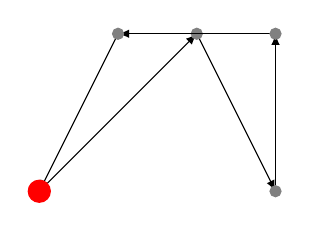
\begin{tikzpicture}
                \draw [black, -latex] (0, 0) -- (2, 2);
                \filldraw [gray] (0, 0) circle (2pt);
                \draw [black, -latex] (2, 2) --(3, 0);
                \filldraw [gray] (2, 2) circle (2pt);
                \draw [black, -latex] (3, 0) --(3, 2);
                \filldraw [gray] (3, 0) circle (2pt);
                \draw [black, -latex] (3, 2) --(1, 2);
                \filldraw [gray] (3, 2) circle (2pt);
                \draw [black, -latex] (1, 2) --(0, 0);
                \filldraw (1, 2) [gray] circle (2pt);
                \filldraw [red] (0, 0) circle (4pt);
            \end{tikzpicture}
        \end{minipage}
        \begin{minipage}{0.5\linewidth}
            % Greedy
            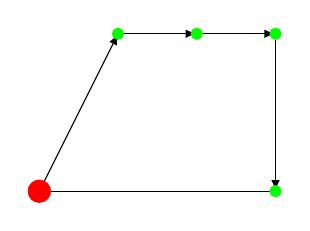
\begin{tikzpicture}
                \draw [black, -latex] (0, 0) -- (1, 2);
                \filldraw [green] (0, 0) circle (2pt);
                \draw [black, -latex] (1, 2) --(2, 2);
                \filldraw [green] (1, 2) circle (2pt);
                \draw [black, -latex] (2, 2) --(3, 2);
                \filldraw [green] (2, 2) circle (2pt);
                \draw [black, -latex] (3, 2) --(3, 0);
                \filldraw [green] (3, 2) circle (2pt);
                \draw [black, -latex] (3, 0) --(0, 0);
                \filldraw (3, 0) [green] circle (2pt);
                \filldraw [red] (0, 0) circle (4pt);
            \end{tikzpicture}
        \end{minipage}

    \end{figure}

    The improvements from the greedy algorithm seem to suggest that it 
    will play an important role in developing our route scheduling 
    algorithm. With this in mind, we attempted explore other local search methods that may be more effective than the greedy approach. One approach we can adopt is based on the opt-2 
    heuristic \cite[p.~457]{cite:eijkhout2022}. The opt-2 heuristic suggests that optimal routes are generally 
    not “entangled” (i.e no intersections). Therefore, if we can work to “detangle” 
    a given list of points we can find its optimal path. Rather than aim to algorithmically identify the intersections in a given path, 
    we can try to “detangle” a path by reversing segments of it and checking to 
    see if such a modification generates a more optimal path. To implement this in code, we employ the follwing strategy:

    % need to fix, there's a better package than fbox that 
    % needs looking into
    \begin{lstlisting} [
        caption=opt2 Algorithm,
        label={lst:opt2_algorithm}
    ]
For all possible segments in our path:
    Make the new path:
        Original start + reversed segment + original end 
        If new path is shorter keep it\end{lstlisting}

        In code this equates to:
        \newpage 
    \begin{lstlisting}[
        language=C++
    ]
Route Route::opt2(){
    AddressList address_list(address_vec);
    double current_length = address_list.length();
    for (int m=1 ; m<address_list.size(); m++){
        for (int n=0; n <= m; n++){
            AddressList new_list(address_list.reverse(n, m+1));
            if ( new_list.length() < address_list.length() ){        
                address_list = new_list;
                current_length = new_list.length();
            } 
        }
    }
    Route new_route(address_list, hub);
    return new_route;
}
\end{lstlisting}

    In this implementation, we utilized the \emph{reverse()} method 
    from the C++ standard library which reverses a given range of a vector 
    in place. Below we compare the results from our greedy algorithm 
    with that of our opt-2 algorithm:

    \begin{figure}[h]
        \caption{Unoptimized Route (black) vs. greedy algorithm (blue) vs. opt-2 algorithm (green) Route is optimized through both the greedy algorithm and the opt2 algorithm. The total distances of each route were 11.76, 11.16, and 11.04 units, for the original, greedy, and opt-2 routes respectively }
        \label{figure:opt2_vs_greedy}
        \begin{minipage}{0.3\linewidth}
            % Old
            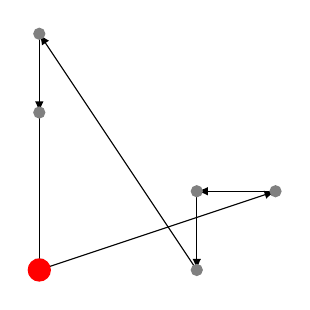
\begin{tikzpicture}
                \draw [black, -latex] (0, 0) -- (3, 1);
                \filldraw [gray] (0, 0) circle (2pt);
                \draw [black, -latex] (3, 1) --(2, 1);
                \filldraw [gray] (3, 1) circle (2pt);
                \draw [black, -latex] (2, 1) --(2, 0);
                \filldraw [gray] (2, 1) circle (2pt);
                \draw [black, -latex] (2, 0) --(0, 3);
                \filldraw [gray] (2, 0) circle (2pt);
                \draw [black, -latex] (0, 3) --(0, 2);
                \filldraw [gray] (0, 3) circle (2pt);
                \draw [black, -latex] (0, 2) --(0, 0);
                \filldraw (0, 2) [gray] circle (2pt);
                \filldraw [red] (0, 0) circle (4pt);
            \end{tikzpicture}
        \end{minipage}
        \begin{minipage}{0.3\linewidth}
            % Greedy
            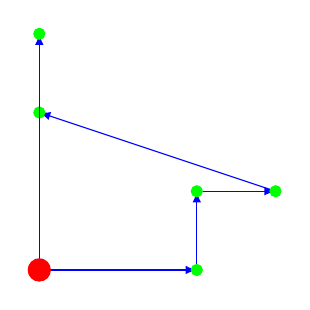
\begin{tikzpicture}
                \draw [blue, -latex] (0, 0) -- (2, 0);
                \filldraw [green] (0, 0) circle (2pt);
                \draw [blue, -latex] (2, 0) --(2, 1);
                \filldraw [green] (2, 0) circle (2pt);
                \draw [blue, -latex] (2, 1) --(3, 1);
                \filldraw [green] (2, 1) circle (2pt);
                \draw [blue, -latex] (3, 1) --(0, 2);
                \filldraw [green] (3, 1) circle (2pt);
                \draw [blue, -latex] (0, 2) --(0, 3);
                \filldraw [green] (0, 2) circle (2pt);
                \draw [blue, -latex] (0, 3) --(0, 0);
                \filldraw (0, 3) [green] circle (2pt);
                \filldraw [red] (0, 0) circle (4pt);
            \end{tikzpicture}
        \end{minipage}
        \begin{minipage}{0.3\linewidth}
            % opt2
            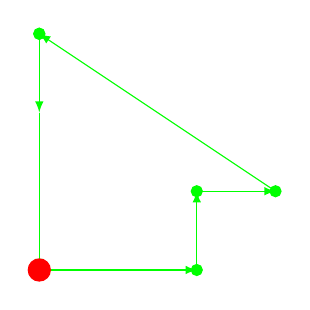
\begin{tikzpicture}
            \draw [green, -latex] (0, 0) -- (2, 0);
            \filldraw [green] (0, 0) circle (2pt);
            \draw [green, -latex] (2, 0) --(2, 1);
            \filldraw [green] (2, 0) circle (2pt);
            \draw [green, -latex] (2, 1) --(3, 1);
            \filldraw [green] (2, 1) circle (2pt);
            \draw [green, -latex] (3, 1) --(0, 3);
            \filldraw [green] (3, 1) circle (2pt);
            \draw [green, -latex] (0, 3) --(0, 2);
            \filldraw [green] (0, 3) circle (2pt);
            \draw [green, -latex] (0, 2) --(0, 0);
            \filldraw (0, 3) [green] circle (2pt);
            \filldraw [red] (0, 0) circle (4pt);
            \end{tikzpicture}
        \end{minipage}
    \end{figure}
    

    The opt-2 algorithm seems to produce slightly better solutions than our 
    greedy algorithm. However, we should also consider this algorithm's 
    efficiency. Calling the \emph{reverse()} and \emph{length()} methods of an 
    \verb|AddressList| of size n leads to an average time complexity of O(n)
    for each. Moreover, because this opt-2 algorithm evaluates a total of 
    \(\frac{n^2}{2}\) combinations.\footnote{The estimation comes from 
    the fact that the total number of combinations is equivalent to the 
    sum of a triangular number sequence.} the overall time complexity of 
    this algorithm is O(2n\textsuperscript3)  which simplifies to 
    O(n\textsuperscript3). Fortunately the efficiency of this algorithm 
    can be slightly improved. Rathan than call \emph{length()} to compare the \emph{total distances} between the 
    modified and original path, we can focus our comparisons on just the 
    \emph{change in distance} caused by each swap.
    Consequently, the time complexity can be reduced, but not to a significant degree (still O(n\textsuperscript3)\footnote{ This comes from the fact that we must still call our \emph{reverse()} method within the nested for-loop, and the \emph{reverse()} which takes on average O(n) time.}). Thus, our opt-2 algorithm seems to be a noticeable 
    improvement from the greedy algorithm at the cost of efficiency. Yet, even this 
    approach may not always produce accurate results. Figure \ref*{figure:opt2_vs_greedy_2} demonstrates this below:
    
    \begin{figure}[h]
        \caption{An unsorted Route is optimized through both the greedy algorithm (blue) and the opt2 algorithm (green).}
        \label{figure:opt2_vs_greedy_2}
        \begin{minipage}{0.3\linewidth}
            % Old
            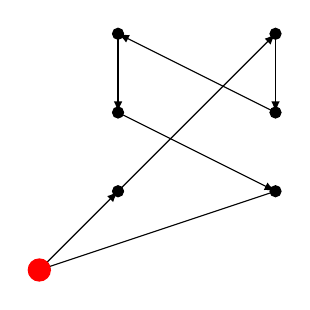
\begin{tikzpicture}
                \draw [black, -latex] (0, 0) -- (1, 1);
                \filldraw [black] (0, 0) circle (2pt);
                \draw [black, -latex] (1, 1) --(3, 3);
                \filldraw [black] (1, 1) circle (2pt);
                \draw [black, -latex] (3, 3) --(3, 2);
                \filldraw [black] (3, 3) circle (2pt);
                \draw [black, -latex] (3, 2) --(1, 3);
                \filldraw [black] (3, 2) circle (2pt);
                \draw [black, -latex] (1, 3) --(1, 2);
                \filldraw [black] (1, 3) circle (2pt);
                \draw [black, -latex] (1, 2) --(3, 1);
                \filldraw [black] (1, 2) circle (2pt);
                \draw [black, -latex] (3, 1) --(0, 0);
                \filldraw (3, 1) [black] circle (2pt);
                \filldraw [red] (0, 0) circle (4pt);
            \end{tikzpicture}
        \end{minipage}
        \begin{minipage}{0.3\linewidth}
            % Greedy
            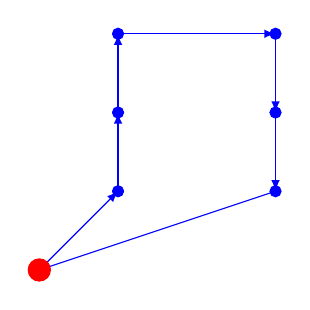
\begin{tikzpicture}
                \draw [blue, -latex] (0, 0) -- (1, 1);
                \filldraw [blue] (0, 0) circle (2pt);
                \draw [blue, -latex] (1, 1) --(1, 2);
                \filldraw [blue] (1, 1) circle (2pt);
                \draw [blue, -latex] (1, 2) --(1, 3);
                \filldraw [blue] (1, 2) circle (2pt);
                \draw [blue, -latex] (1, 3) --(3, 3);
                \filldraw [blue] (1, 3) circle (2pt);
                \draw [blue, -latex] (3, 3) --(3, 2);
                \filldraw [blue] (3, 3) circle (2pt);
                \draw [blue, -latex] (3, 2) --(3, 1);
                \filldraw [blue] (3, 2) circle (2pt);
                \draw [blue, -latex] (3, 1) --(0, 0);
                \filldraw (3, 1) [blue] circle (2pt);
                \filldraw [red] (0, 0) circle (4pt);
            \end{tikzpicture}
        \end{minipage}
        \begin{minipage}{0.3\linewidth}
            % opt2
            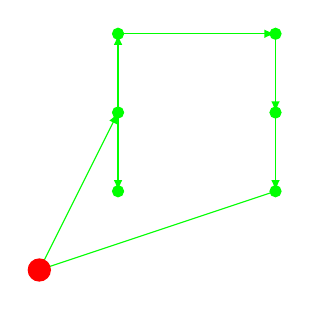
\begin{tikzpicture}
                \draw [green, -latex] (0, 0) -- (1, 2);
                \filldraw [green] (0, 0) circle (2pt);
                \draw [green, -latex] (1, 2) --(1, 1);
                \filldraw [green] (1, 2) circle (2pt);
                \draw [green, -latex] (1, 1) --(1, 3);
                \filldraw [green] (1, 1) circle (2pt);
                \draw [green, -latex] (1, 3) --(3, 3);
                \filldraw [green] (1, 3) circle (2pt);
                \draw [green, -latex] (3, 3) --(3, 2);
                \filldraw [green] (3, 3) circle (2pt);
                \draw [green, -latex] (3, 2) --(3, 1);
                \filldraw [green] (3, 2) circle (2pt);
                \draw [green, -latex] (3, 1) --(0, 0);
                \filldraw (3, 1) [green] circle (2pt);
                \filldraw [red] (0, 0) circle (4pt);
            \end{tikzpicture}
        \end{minipage}
    \end{figure}

    Thus, to develop more optimal solutions we could choose to employ our 
    greedy algorithm followed by opt-2. Using both algorithms would lead to a time complexity of O(n\textsuperscript2 + n\textsuperscript3), so the overall time complexity would be O(n\textsuperscript3). Due to having a larger overall time complexity, it may be more effective to only use our greedy algorithm when optimizing routes. Moreover, although this approach is well-suited for single delivery routes, 
    we may also wish to extend the opt-heuristic to optimize two routes simultaneously. In other words, we may wish to further shorten the paths of two routes 
    by swapping segments of one route out for segments of another. This may be more 
    desirable, as it introduces more flexibility, and thus could lead to identifying 
    potentially shorter paths.



    \subsection{Multiple Traveling Salesmen Problem}
    \label{subsection:Multiple_Traveling_Salesmen_Problem}
    
    Optimizing multiple routes simultaneously extends our 
    Traveling Salesman Problem to the Multiple Travelling 
    Salesman Problem (MTSP). Seeing how computationally 
    expensive our initial opt2 algorithm was in section 
    \ref{subsection:Traveling_Salesman_Problem} , one can imagine how much greater 
    this costs would become for an algorithm that optimized 
    multiple routes simeltaneously. For this reason, and 
    others we will, aim to optimize only two routes at 
    once. As mentioned in section \ref{subsection:Traveling_Salesman_Problem} we can achieve this 
    by extending the opt-2 heuristic to multiple routes, as seen in Listing \ref{lst:opt2_multi_algorithm}
    
    % fix this work like a numbered list
    \begin{lstlisting} [
        caption=opt2 Multi Algorithm,
        label={lst:opt2_multi_algorithm}
    ]
For all possible segments for both routes
    swap both routes with the following variations:
        1. Reverse route 1 then swap
        2. Reverse route 2 then swap
        3. Just swap
        4. Reverse both routes then swap
    If the distance from any of the variations is improved
        keep the modification.\end{lstlisting}
    
    
    As mentioned previously in this section, 
    we can expect the time complexity of this algorithm 
    to be larger than that of the single route opt-2 algorithm. 
    The multi-path opt-2 algorithm uses four for-loops 
    (two for each route). Further, at each iteration 
    of the innermost loop, we call our reverse and swap 
    methods several times. Both methods have a time
     complexity of O(n) (where n is the number of 
     addresses in each route). Since those methods 
     are called in total nine times, the time complexity 
     of the innermost loops is O(9n) which simplifies to O(n).
     Consequently, when we consider our four for-loops 
     the overall time complexity becomes O(n\textsuperscript5).
     \footnote{Futhermore, the time complexity would be 
     O(m\textsuperscript5+n\textsuperscript5) If we consider 
     routes of differing lengths m and n.} It’s important to 
     note that the time complexity of this algorithm 
     can also be improved, but at a cost. For example, 
     two for-loops are created to account for total 
     possible starting and ending of each segment per 
     route. To improve runtime, we could simply give 
     each segment a fixed length, thereby reducing 
     the time complexity to O(n\textsuperscript3). However, 
     this comes at the cost of accuracy, as our algorithm 
     may ignore more optimal solutions due to this constraint. 
     Therefore, therein lies a tradeoff between accuracy and 
     efficiency that we must consider when choosing which 
     approach/algorithm to use. 

    In prioritizing accuracy, we will choose to pay the computational costs and use a multi-path-op2 algorithm that swaps segments of varied lengths. Additionally, we can also choose to use this algorithm to optimize two routes belonging to a single driver (that is, spread over two different days). In this case, we may also want to consider optimizing for the total distance traveled by both routes, rather than the \emph{individual} distance traveled by both routes. The figures below demonstrate how this subtle change in constraints produces dramatically different results:
    \begin{figure}[h]
        \caption{Two Routes exchange Addresses to optimize the total distance from 19.62 to 16.51}
        \label{figure:swap_1}
        \begin{minipage}{0.45\linewidth}
            % Unswapped
            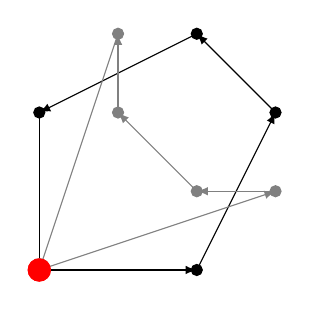
\begin{tikzpicture}
                % Route 1
                \draw [black, -latex] (0, 0) -- (2, 0);
                \filldraw [black] (0, 0) circle (2pt);
                \draw [black, -latex] (2, 0) --(3, 2);
                \filldraw [black] (2, 0) circle (2pt);
                \draw [black, -latex] (3, 2) --(2, 3);
                \filldraw [black] (3, 2) circle (2pt);
                \draw [black, -latex] (2, 3) --(0, 2);
                \filldraw [black] (2, 3) circle (2pt);
                \draw [black, -latex] (0, 2) --(0, 0);
                \filldraw (0, 2) [black] circle (2pt);
                \filldraw [red] (0, 0) circle (4pt);
                % Route 2
                \draw [gray, -latex] (0, 0) -- (3, 1);
                \filldraw [gray] (0, 0) circle (2pt);
                \draw [gray, -latex] (3, 1) --(2, 1);
                \filldraw [gray] (3, 1) circle (2pt);
                \draw [gray, -latex] (2, 1) --(1, 2);
                \filldraw [gray] (2, 1) circle (2pt);
                \draw [gray, -latex] (1, 2) --(1, 3);
                \filldraw [gray] (1, 2) circle (2pt);
                \draw [gray, -latex] (1, 3) --(0, 0);
                \filldraw (1, 3) [gray] circle (2pt);
                \filldraw [red] (0, 0) circle (4pt);
            \end{tikzpicture}
        \end{minipage}
        \begin{minipage}{0.45\linewidth}
            % Swapped
            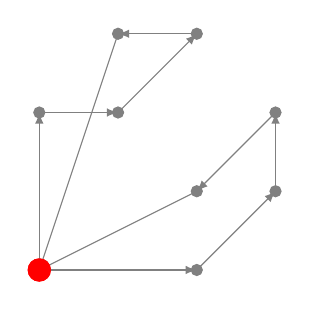
\begin{tikzpicture}
                % Route 1
                \draw [gray, -latex] (0, 0) -- (2, 0);
                \filldraw [gray] (0, 0) circle (2pt);
                \draw [gray, -latex] (2, 0) --(3, 1);
                \filldraw [gray] (2, 0) circle (2pt);
                \draw [gray, -latex] (3, 1) --(3, 2);
                \filldraw [gray] (3, 1) circle (2pt);
                \draw [gray, -latex] (3, 2) --(2, 1);
                \filldraw [gray] (3, 2) circle (2pt);
                \draw [gray, -latex] (2, 1) --(0, 0);
                \filldraw (2, 1) [gray] circle (2pt);
                \filldraw [red] (0, 0) circle (4pt);
                % Route 2
                \draw [gray, -latex] (0, 0) -- (0, 2);
                \filldraw [gray] (0, 0) circle (2pt);
                \draw [gray, -latex] (0, 2) --(1, 2);
                \filldraw [gray] (0, 2) circle (2pt);
                \draw [gray, -latex] (1, 2) --(2, 3);
                \filldraw [gray] (1, 2) circle (2pt);
                \draw [gray, -latex] (2, 3) --(1, 3);
                \filldraw [gray] (2, 3) circle (2pt);
                \draw [gray, -latex] (1, 3) --(0, 0);
                \filldraw (1, 3) [gray] circle (2pt);
                \filldraw [red] (0, 0) circle (4pt);
            \end{tikzpicture}
        \end{minipage}
    \end{figure}
    \begin{figure}[h]
        \caption{Two Routes exchange Addresses to optimize their individual distance from 9.88 and 9.73 units to 9.81 and 8.58 units respectively.}
        \label{figure:swap_2}
        \begin{minipage}{0.45\linewidth}
            % Unswapped
            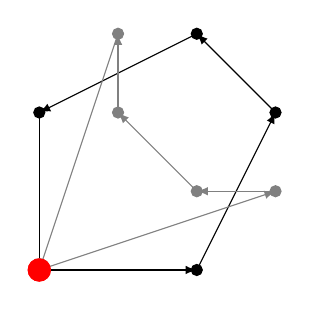
\begin{tikzpicture}
                % Route 1
                \draw [black, -latex] (0, 0) -- (2, 0);
                \filldraw [black] (0, 0) circle (2pt);
                \draw [black, -latex] (2, 0) --(3, 2);
                \filldraw [black] (2, 0) circle (2pt);
                \draw [black, -latex] (3, 2) --(2, 3);
                \filldraw [black] (3, 2) circle (2pt);
                \draw [black, -latex] (2, 3) --(0, 2);
                \filldraw [black] (2, 3) circle (2pt);
                \draw [black, -latex] (0, 2) --(0, 0);
                \filldraw (0, 2) [black] circle (2pt);
                \filldraw [red] (0, 0) circle (4pt);
                % Route 2
                \draw [gray, -latex] (0, 0) -- (3, 1);
                \filldraw [gray] (0, 0) circle (2pt);
                \draw [gray, -latex] (3, 1) --(2, 1);
                \filldraw [gray] (3, 1) circle (2pt);
                \draw [gray, -latex] (2, 1) --(1, 2);
                \filldraw [gray] (2, 1) circle (2pt);
                \draw [gray, -latex] (1, 2) --(1, 3);
                \filldraw [gray] (1, 2) circle (2pt);
                \draw [gray, -latex] (1, 3) --(0, 0);
                \filldraw (1, 3) [gray] circle (2pt);
                \filldraw [red] (0, 0) circle (4pt);
            \end{tikzpicture}
        \end{minipage}
        \begin{minipage}{0.45\linewidth}
            % Unswapped
            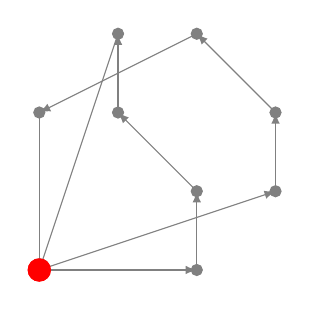
\begin{tikzpicture}
                % Route 1
                \draw [gray, -latex] (0, 0) -- (3, 1);
                \filldraw [gray] (0, 0) circle (2pt);
                \draw [gray, -latex] (3, 1) --(3, 2);
                \filldraw [gray] (3, 1) circle (2pt);
                \draw [gray, -latex] (3, 2) --(2, 3);
                \filldraw [gray] (3, 2) circle (2pt);
                \draw [gray, -latex] (2, 3) --(0, 2);
                \filldraw [gray] (2, 3) circle (2pt);
                \draw [gray, -latex] (0, 2) --(0, 0);
                \filldraw (0, 2) [gray] circle (2pt);
                \filldraw [red] (0, 0) circle (4pt);
                % Route 2
                \draw [gray, -latex] (0, 0) -- (2, 0);
                \filldraw [gray] (0, 0) circle (2pt);
                \draw [gray, -latex] (2, 0) --(2, 1);
                \filldraw [gray] (2, 0) circle (2pt);
                \draw [gray, -latex] (2, 1) --(1, 2);
                \filldraw [gray] (2, 1) circle (2pt);
                \draw [gray, -latex] (1, 2) --(1, 3);
                \filldraw [gray] (1, 2) circle (2pt);
                \draw [gray, -latex] (1, 3) --(0, 0);
                \filldraw (1, 3) [gray] circle (2pt);
                \filldraw [red] (0, 0) circle (4pt);
            \end{tikzpicture}
        \end{minipage}
    \end{figure}

    \newpage
    Notice how in Figure \ref*{figure:swap_1} we achieve a smaller \emph{total} distance at the expense of increasing the \emph{individual distance} of route 1 of the routes. Whereas in Figure \ref*{figure:swap_2} we optimize for the \emph{individual distances} of each route at the expense of having a larger \emph{total distance} (from taking the sum of both routes). As a result, it seems we may want to optimize for total distance and individual distance on a case-by-case basis. For example, in the scenario of scheduling routes for multiple (in this case two) truck drivers it may seem more logical to optimize for individual distances. This is because having lopsided routes similar to that shown in Figure \ref*{figure:swap_2} can lead to undelivered packages (in the event that one route is so long all points cannot be visited in a single shift of work). Conversely, in the scenario that we were trying to optimize two routes belonging to the same truck driver, it seems more logical to optimize for total distance traveled across both routes (although this is assuming delivery timing is not a factor)\footnote{this is because swapping segments containing different delivery times would lead to some packages being delivered early while others being delivered too late. We don't mind early deliveries, but late deliveries are unacceptable.}. For our final product, we will take these factors into account to strategically optimize routes for truck drivers using the algorithms discussed.
    
    % Talk about how swap algorithm works. Figure \ref{figure:swapdemo} provides a simple example of how this algorithm improves the total distance. (Now prove it with data! What are the distances before and after?) ALSO: Talk about how the gray and black Addresses are symmetrical, but the trucks take different Routes. Is this okay, or does one or both of them need to go through greedy/opt2???



    \subsection{Developing the Final Product}
    \label{subsection:Developing_the_Final_Product}
    After our team implemented our solutions to the Single and Multiple Traveling Salesman Problems, we decided to explore dynamicism by constructing a simplified route allocator for a delivery company. Every morning, a regional fulfilment center recives a list of orders to fulfill, corresponding to packages available onsite. It invokes our program, which combines these with unfulfilled orders from the previous day, and delegates them amongst a predetermined number of trucks. The \verb|Route|s are then optimized individually and between one another. At this point, their distances are measured. If a \verb|Route| exceeds a predetermined distance limit, \verb|Address|es are removed from the \verb|Route| based on their \verb|deliver_by| due date, until it falls within an acceptable length. The delivery routes are then exported to documents for the drivers, the unfulfilled orders are saved to a file which overwrites the old one, and performance statistics are compiled into a report for management.

    All of the tasks to be completed before the start of a business day are modularized in a single function. It requires parameters specifying input and output file locations, the number of trucks available, the maximum permissible route distance, the hub address, and a boolean which allows the user to specify if data should be output from intermediate optimization steps. Most of the harder tasks of the simulation have already been solved in our library. This even includes the repetitive tasks of reading or exporting a \verb|Route| or \verb|AddressList| from or to a file, based on a given file path string. To demonstrate this program, we constructed a simulation with 18 pre-generated daily orders spanning 9 days.
    
    In addition, we used a pared-down version, with limited file output, to experiment with variations in simulation parameters. Each simulation is a sigle data point, drawing from 20 daily orders across 30 days. The same order data was used for each data point. The nature and results of these simulations are discussed in Section \ref{section:Results}.

    \section{Results}
    \label{section:Results}
    % Pretty pictures and tables go here. Describe each situation being displayed and talk about what they mean, e.g. is it the optimal solution? Good enough? Is there a tradeoff between time to execute and quality of results?

    % Hmm, maybe insert a table comparing number of nodes/trucks to program execution time. What rate does it increase at $(O(n), O(n^2), \&c.)$

    For our main simulation, we generated randomized order data spanning 9 days. Each day has 18 orders with coordinates spanning from 0 to 10 excluding the hub, i.e. $\{ (i, j) \in \mathbb{Z}^2 | 0 \leq i \leq 10 \cap 0 \leq j \leq 10\} - \{ (0, 0)\}$. Delivery due dates range from 1 to 7 days after the order was generated. For this test, 3 trucks were used, and the distance limit was set to 35.0 for each truck. The resulting outputs, spread across over 100 data files, would be quite tedious to present in full in this report, so the results will be condensed into tables and figures. To view samples of each form of output, please refer to Appendix \ref{appendix:Sample_Output_Files}.

    The first thing to consider from the results is whether the optimization performed as expected. As seen in Figure \ref{figure:day1opt}, stops are exchanged within and between truck routes until they all take efficient paths. Since no orders were left undelivered on Day 1, all of the Addresses are still present afterwards. This can be verified for the other days as well.

    \begin{figure}[h]
        \caption{Day 1 Optimization, Before and After}
        \label{figure:day1opt}
        \begin{minipage}{0.45\linewidth}
            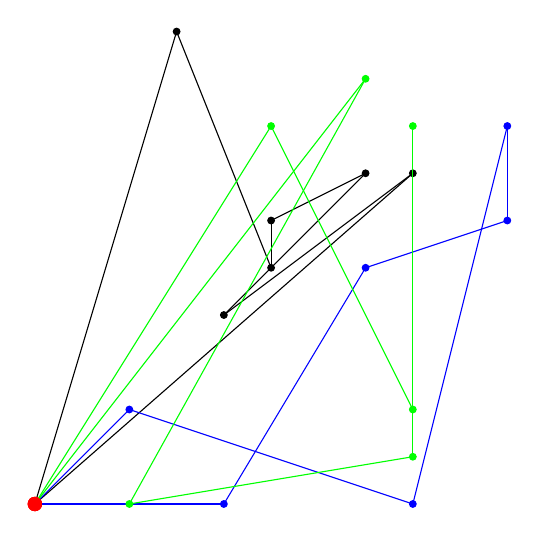
\begin{tikzpicture}[scale=0.6]
                % Truck 1
                \draw [black] (0, 0) -- (8, 7);
                \filldraw [black] (0, 0) circle (2pt);
                \draw [black] (8, 7) --(4, 4);
                \filldraw [black] (8, 7) circle (2pt);
                \draw [black] (4, 4) --(7, 7);
                \filldraw [black] (4, 4) circle (2pt);
                \draw [black] (7, 7) --(5, 6);
                \filldraw [black] (7, 7) circle (2pt);
                \draw [black] (5, 6) --(5, 5);
                \filldraw [black] (5, 6) circle (2pt);
                \draw [black] (5, 5) --(3, 10);
                \filldraw [black] (5, 5) circle (2pt);
                \draw [black] (3, 10) --(0, 0);
                \filldraw (3, 10) [black] circle (2pt);
                \filldraw [red] (0, 0) circle (4pt);
                % Truck 2
                \draw [blue] (0, 0) -- (4, 0);
                \filldraw [blue] (0, 0) circle (2pt);
                \draw [blue] (4, 0) --(7, 5);
                \filldraw [blue] (4, 0) circle (2pt);
                \draw [blue] (7, 5) --(10, 6);
                \filldraw [blue] (7, 5) circle (2pt);
                \draw [blue] (10, 6) --(10, 8);
                \filldraw [blue] (10, 6) circle (2pt);
                \draw [blue] (10, 8) --(8, 0);
                \filldraw [blue] (10, 8) circle (2pt);
                \draw [blue] (8, 0) --(2, 2);
                \filldraw [blue] (8, 0) circle (2pt);
                \draw [blue] (2, 2) --(0, 0);
                \filldraw (2, 2) [blue] circle (2pt);
                \filldraw [red] (0, 0) circle (4pt);
                % Truck 3
                \draw [green] (0, 0) -- (5, 8);
                \filldraw [green] (0, 0) circle (2pt);
                \draw [green] (5, 8) --(8, 2);
                \filldraw [green] (5, 8) circle (2pt);
                \draw [green] (8, 2) --(8, 8);
                \filldraw [green] (8, 2) circle (2pt);
                \draw [green] (8, 8) --(8, 1);
                \filldraw [green] (8, 8) circle (2pt);
                \draw [green] (8, 1) --(2, 0);
                \filldraw [green] (8, 1) circle (2pt);
                \draw [green] (2, 0) --(7, 9);
                \filldraw [green] (2, 0) circle (2pt);
                \draw [green] (7, 9) --(0, 0);
                \filldraw (7, 9) [green] circle (2pt);
                \filldraw [red] (0, 0) circle (4pt);
            \end{tikzpicture}
        \end{minipage}
        \begin{minipage}{0.45\linewidth}
            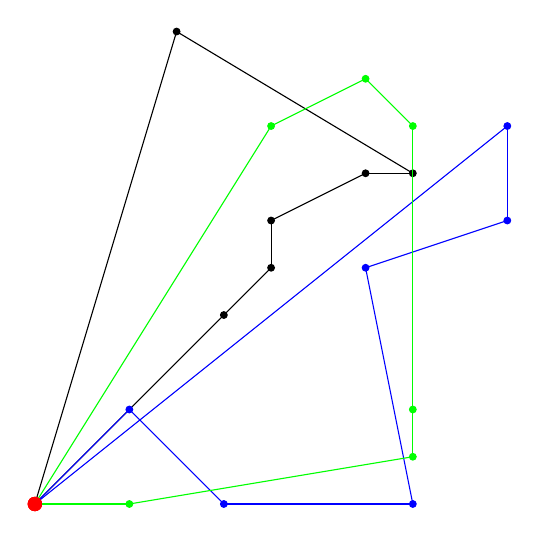
\begin{tikzpicture}[scale=0.6]
                % Truck 1
                \draw [black] (0, 0) -- (4, 4);
                \filldraw [black] (0, 0) circle (2pt);
                \draw [black] (4, 4) --(5, 5);
                \filldraw [black] (4, 4) circle (2pt);
                \draw [black] (5, 5) --(5, 6);
                \filldraw [black] (5, 5) circle (2pt);
                \draw [black] (5, 6) --(7, 7);
                \filldraw [black] (5, 6) circle (2pt);
                \draw [black] (7, 7) --(8, 7);
                \filldraw [black] (7, 7) circle (2pt);
                \draw [black] (8, 7) --(3, 10);
                \filldraw [black] (8, 7) circle (2pt);
                \draw [black] (3, 10) --(0, 0);
                \filldraw (3, 10) [black] circle (2pt);
                \filldraw [red] (0, 0) circle (4pt);
                % Truck 2
                \draw [blue] (0, 0) -- (2, 2);
                \filldraw [blue] (0, 0) circle (2pt);
                \draw [blue] (2, 2) --(4, 0);
                \filldraw [blue] (2, 2) circle (2pt);
                \draw [blue] (4, 0) --(8, 0);
                \filldraw [blue] (4, 0) circle (2pt);
                \draw [blue] (8, 0) --(7, 5);
                \filldraw [blue] (8, 0) circle (2pt);
                \draw [blue] (7, 5) --(10, 6);
                \filldraw [blue] (7, 5) circle (2pt);
                \draw [blue] (10, 6) --(10, 8);
                \filldraw [blue] (10, 6) circle (2pt);
                \draw [blue] (10, 8) --(0, 0);
                \filldraw (10, 8) [blue] circle (2pt);
                \filldraw [red] (0, 0) circle (4pt);
                % Truck 3
                \draw [green] (0, 0) -- (2, 0);
                \filldraw [green] (0, 0) circle (2pt);
                \draw [green] (2, 0) --(8, 1);
                \filldraw [green] (2, 0) circle (2pt);
                \draw [green] (8, 1) --(8, 2);
                \filldraw [green] (8, 1) circle (2pt);
                \draw [green] (8, 2) --(8, 8);
                \filldraw [green] (8, 2) circle (2pt);
                \draw [green] (8, 8) --(7, 9);
                \filldraw [green] (8, 8) circle (2pt);
                \draw [green] (7, 9) --(5, 8);
                \filldraw [green] (7, 9) circle (2pt);
                \draw [green] (5, 8) --(0, 0);
                \filldraw (5, 8) [green] circle (2pt);
                \filldraw [red] (0, 0) circle (4pt);
            \end{tikzpicture}
        \end{minipage}
    \end{figure}

    Reports and data files can also be examined for their accuracy; refer to Listings \ref{lst:Sample_Data_File} and \ref{lst:Sample_TikZ_File} to see that they correspond to the black unsorted route. On the other hand, the job assignment in Listing \ref{lst:Sample_Job_Assignment} corresponds to the black sorted route, and the order numbers in the status report in Listing \ref{lst:Sample_Satus_Report} match the number of stops and distances of the sorted routes.

    From there, we can study the numbers provided in the status reports. Delivery fulfillment statistics are condensed into Table \ref{table:deliverystats}. We can utilize this to analyze the hub's performance. In general, the hob is keeping up with the order inflow rate. Some days it isn't able to deliver everything, but it eventually catches up. This could be an important experimental metric for a delivery organization. Parameters like the number of trucks and the maximum delivery distance could be adjusted to find critical points where orders get added to the backlog faster than they are removed.

    \begin{table}[h]
        \centering
        \caption{Status Report Output Data}
        \label{table:deliverystats}
        \begin{tabular}{cccccccc}
            & \multicolumn{3}{c}{Delivered} && \multicolumn{3}{c}{Undelivered} \\
            & Early & On Time & Late && Not Due & Due Tomorrow & Overdue \\
            \cline{2-4} \cline{6-8}
            Day 1 & 18 & 0 & 0 && 0 & 0 & 0 \\
            Day 2 & 16 & 0 & 0 && 0 & 0 & 0 \\
            Day 3 & 10 & 0 & 0 && 8 & 0 & 0 \\
            Day 4 & 16 & 0 & 0 && 7 & 0 & 0 \\
            Day 5 & 16 & 0 & 0 && 6 & 0 & 0 \\
            Day 6 & 23 & 0 & 0 && 0 & 0 & 0 \\
            Day 7 & 12 & 0 & 0 && 4 & 0 & 0 \\
            Day 8 & 19 & 0 & 0 && 1 & 0 & 0 \\
            Day 9 & 17 & 0 & 0 && 1 & 0 & 0 \\
        \end{tabular}
    \end{table}

    At this point, the main problem is solved. For a given list of orders, our program can find an optimal solution within a certain distance range and eliminate low-priority orders to keep delivery routes within a certain distance constraint. Now we will extend our investigation into modifying parameters of the simulation. As mentioned before, at a certain point, the simulation will likely start backlogging orders. If we find this point, managers could leverage it to maximize efficiency while maintaining customer satisfaction. In Section \ref{subsection:Varying_the_Distance_Limit}, we investigate how varying the maximum permissible route distance impacts backlogs. In section \ref{subsection:Varying_the_Number_of_Trucks_Deployed}, we investigate how varying the number of trucks deployed impacts backlogs. Finally, in Section \ref{subsection:Performance_Data}, we briefly reflect on the execution times of the programs.

    \subsection{Varying the Distance Limit}
    \label{subsection:Varying_the_Distance_Limit}
    First, we consider varying the distance limit for each truck. Note that for a delivery zone ranging from coordinates 0 to $d$ with a hub at $(0, 0)$, if the distance limit were dropped below $2 * d \sqrt{2}$, then some orders would be forever out of range. This sets a lower limit for our maximum permissible distance at $2 \cdot 10 \sqrt{2} \approx 28.28$. However, because there are more orders for the hub to process than trucks, the limit will likely be higher. Figure \ref{img:experiment1} shows that for 3 trucks receiving 20 orders per day in a 10-by-10 grid, orders start to maintain a constant backlog below a minimum distance of 34. After that point, unfulfilled orders climb signigicantly. Interestingly, after an initial climb, backlogs tend to level off. The exact cause of this would require more investigation, but it's possible that once the backlog is high, it is counteracted by new orders occurring at the same locations as old ones, thus being merged.

    \begin{figure}[h]
        \centering
        \caption{The order backlog builds up as the route distance limit drops below 34.}
        \label{img:experiment1}
        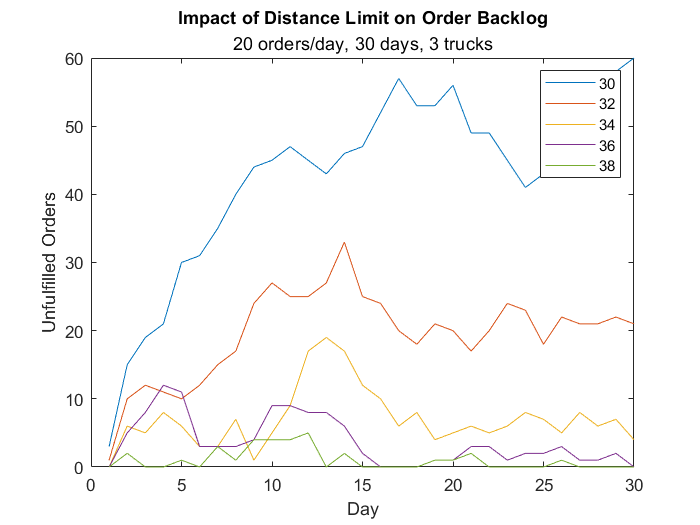
\includegraphics[width=\textwidth]{experiment1.png}
    \end{figure}

    \subsection{Varying the Number of Trucks Deployed}
    \label{subsection:Varying_the_Number_of_Trucks_Deployed}
    Now, we consider varying the number of trucks. Obviously, a delivery company would be interested in minimizing the number of trucks it has to deploy. A similar experiment was conducted on the same data as before. Here, we find a more striking threshold. Figure \ref{img:experiment2} shows that once the number of trucks drops below 3, the backlog explodes, albeit with a similar leveling-off as before. What this means is that the delivery company could not get away with short-staffing for very long before being overwhelmed.

    \begin{figure}[h]
        \centering
        \caption{The order backlog builds up as the number of trucks deployed drops below 3.}
        \label{img:experiment2}
        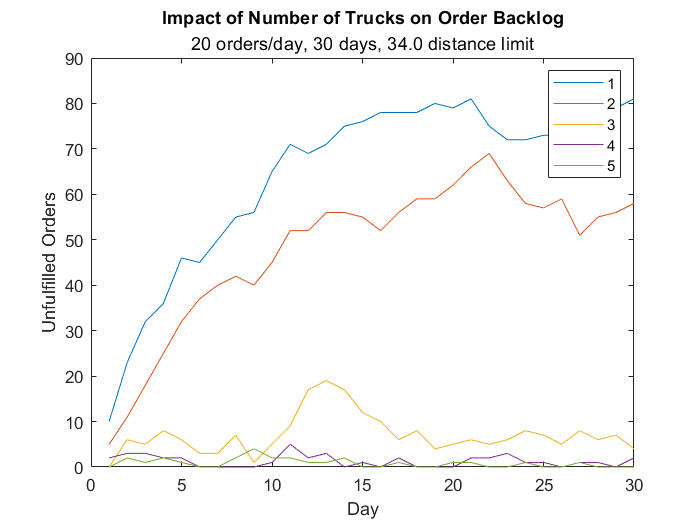
\includegraphics[width=\textwidth]{experiment2.png}
    \end{figure}

    \subsection{Performance Data}
    \label{subsection:Performance_Data}
    Finally, for each of the simulations, i.e. our main program and our experimental one, we recorded the total execution time both on a laptop computer and on the ISP machine. Our main program took 795 milliseconds on a laptop and 75 milliseconds on the supercomputer. The experimental series took 958,455 and 199,371 milliseconds, respectively. Clearly, the supercomputer offers a significant speed advantage in carrying out the programs.

    \section{Conclusion}
    \label{section:Conclusion}
    There are ways to improve the simulation but there are also flaws to consider. For example, the address removal isn’t intelligent, meaning it’s only purely by date and doesn't consider anything else. Also, orders aren’t held back to be grouped with later-arriving orders which hurts efficiency. Another flaw is that when a driver completes an order, stops are removed without the route being reoptimized. Also, there isn’t a friendly user interface for ease of use, which is inconvenient for non tech-savvy people to interface with it. Finally, overall the main simulation program isn’t very flexible; for example, to change the document names and formatting, one has to go into the code, and dat files have to be in a specific format and can’t be a database. This impacts efficiency, which will harm order completion and delivery time, and can be improved in future studies. 

    Ethics is a big concern in the delivery industry because there have been multiple discussions and investigations of working conditions and overloading drivers with too many orders with no breaks. In fact, one source said 50-80\% of workers were pushed to work harder, experienced psychological stress and physical pain \cite{cite:pasternack2019}. One concern of our program is managers could use it to push the limits of workers. When companies are thinking about liability, this becomes crucial because if these drivers are overworked and tired on the road, there is a greater probability of car accidents. The company would have to take responsibility for accidents and possible suing; thus, the safer thing to do would be to make sure we give these drivers more grace and time to breathe. Our program could budget time  for gas and lunch breaks for drivers when assigning orders so that workers aren’t overworked.

    We can use several ideas to improve and scale up the Traveling Salesman Problem. For example, one could create a boolean marking if an order is part of the prime service. This application would enable the order to have some sort of priority over orders that are due earlier but aren’t prime. Furthermore, when drivers are working in urban areas, traffic and common car accidents and road closures in the city is something to consider and be implemented in the program using navigation data from tools such as Waze and Google Maps. Other aspects to consider are speed limits and types of environments, such as delivering an extremely high volume of orders in dense metropolitan areas where streets are hard to navigate. 

    Additionally, companies are now adding online groceries as an option, like the collaboration between Wholefoods and Amazon called Amazon Fresh. One could take this study further by designing the program to prioritize orders for perishable items with a small shell life. Lastly, multiple apartment complexes accept packages only during office or lobby hours. For example, Grandmarc Austin Student Living closes each day between 4-5. Therefore, if an order has an expected delivery time of 8 pm, then the driver who goes to drop it off will not be able to complete the order on that day. They will have to return to attempt to complete that order the next day which wastes time, fuel, and ultimately money. Thus, one could further revise the program to consider if the address is located in a secured complex, and what the policies and hours of operation are to reduce wasting time if drivers cannot complete orders due to office hours. 

    Throughout the process of completing this exploration, we were able to gain experience and learn about scientific management and how to be very precise when managing a business with simulations. In this case, we discovered how to deliver the best route, but also decided how many trucks to deploy, and how to cut costs and time for delivery parcels. Furthermore, we learned about many other aspects to consider when thinking of ethics and wondered how limiting the number of trucks will burden drivers and how we can address this issue. Ultimately, we learned how integrated and complicated the structure of a business is when trying to optimize production while also having to consider so many other factors. 

    \appendix
    \section{Sample Output Files}
    \label{appendix:Sample_Output_Files}

    A variety of data files are used as inputs, intermediates, and outputs of our main program and scripts. They fall into 4 main categories. Data files like Listing \ref{lst:Sample_Data_File} are used to input Addresses into the program and save output Routes from the program. The example is clearly a Route, since it starts and ends at the same location, in this case, the origin. TikZ files like Listing \ref{lst:Sample_TikZ_File} are used to automate plotting figures with the TikZ package in \LaTeX . Job assignments like Listing \ref{lst:Sample_Job_Assignment} format Routes such that human drivers can read them. They also offer some statistics and custom messages. In this case, an affirmation is distributed to drivers to increase morale. Finally, status reports like Listing \ref{lst:Sample_Satus_Report} condense essential information like delivery numbers for managers to evaluate the hub's performance.

    \lstinputlisting[caption=Sample Data File, label={lst:Sample_Data_File}]{day1_truck1_v0.dat}

    \lstinputlisting[caption=Sample TikZ File, label={lst:Sample_TikZ_File}]{day1_truck1_v0.tikz}

    \lstinputlisting[caption=Sample Job Assignment, label={lst:Sample_Job_Assignment}]{day1_truck1.txt}

    \lstinputlisting[caption=Sample Status Report, label={lst:Sample_Satus_Report}]{day1_status.txt}

    \bibliographystyle{plain}
    \bibliography{ref}
\end{document}